\documentclass[10pt,letterpaper]{article}

\usepackage{amsmath,amssymb}
\usepackage{graphicx}
\usepackage[utf8]{inputenc}
\usepackage[T1]{fontenc}
\usepackage[margin=1in]{geometry}
\usepackage{booktabs}
\usepackage{hyperref}
\usepackage{lineno}
\usepackage{authblk}
\usepackage{caption}
\usepackage{xcolor}
\usepackage{natbib}

\linenumbers

\graphicspath{{../benchmarks/}{../analysis/1kg_chr21/results/}{../analysis/1kg_chr21/selection_scan/}{../}}

\title{Coalescence by exhaustion: GPU-accelerated pairwise TMRCA reveals population-specific selection signals in the 1000 Genomes}

\author[1]{Kevin Korfmann}
\author[1]{Sara Mathieson}
\affil[1]{Department of Biology, University of Pennsylvania, Philadelphia, PA, USA}

\date{}

\begin{document}

\maketitle

% ============================================================================
\begin{abstract}
Pairwise coalescence times (TMRCAs) at each genomic position encode the full genealogical history between haplotypes, but estimating them for all pairs in a population sample has been computationally intractable.
Here we present \texttt{tmrca.cu}, a GPU implementation of the Gamma-SMC forward--backward algorithm that reduces pairwise TMRCA inference by two to three orders of magnitude relative to existing CPU methods, while simultaneously improving accuracy through a full forward--backward posterior ($r = 0.820$ versus $r = 0.791$ for the forward-only estimate).
We apply \texttt{tmrca.cu} to 3{,}202 individuals from the 1000 Genomes Project across chromosome~21, computing 829{,}638 within-population pairwise TMRCA profiles over 1{,}002{,}753 segregating sites in 13 minutes on three NVIDIA A100 GPUs.
Aggregating per-site estimates into 214 protein-coding genes and adopting an analytical framework from single-cell genomics---where haplotype pairs are observations and genes are features---we show that population structure emerges directly from TMRCA variation.
By ranking genes within each population independently, we separate gene-specific selection signals from the demographic background, identifying candidates for recent selective sweeps including \textit{CFAP298} in Vietnamese (KHV, 5th within-population percentile) and \textit{KRTAP21-3} in Peruvian (PEL, 6th percentile) individuals.
Supervised UMAP on the top rank-outlier genes amplifies these population-specific signals, producing clean separation of continental groups from a single chromosome's TMRCA data alone.
These results establish exhaustive pairwise TMRCA as a tractable, information-rich data modality for population-scale genomic analysis.
\end{abstract}

% ============================================================================
\section*{Author Summary}
Every pair of individuals shares a common ancestor at every position in the genome.
The time to that ancestor---the TMRCA---varies along the genome and between populations, shaped by recombination, drift, migration, and natural selection.
Computing these coalescence times for all pairs in a large cohort has been too slow to be practical: existing methods process one pair at a time on CPU.
We developed \texttt{tmrca.cu}, a GPU tool that makes this computation fast enough to treat pairwise TMRCA as a new kind of population-scale data---analogous to how gene expression is used in single-cell biology.
Applied to 3{,}202 individuals from the 1000 Genomes Project, we compute over 800{,}000 pairwise TMRCA profiles in 13 minutes and show that the resulting data reveals population structure, identifies genes under selection, and separates demographic history from gene-specific evolutionary signals.

% ============================================================================
\section*{Introduction}

The time to the most recent common ancestor (TMRCA) between a pair of haplotypes is one of the most information-rich summaries of their shared genealogical history.
At each position along the genome, the pairwise coalescence time reflects the local genealogy shaped by recombination, mutation, drift, migration, and natural selection \cite{Li2011,Schiffels2014}.
A complete matrix of pairwise TMRCAs across all sites and all pairs in a sample would provide a rich substrate for population genetic analyses: demographic inference, detection of selective sweeps, estimation of local effective population size, and identification of identity-by-descent segments \cite{Palamara2012,Ralph2013,Kelleher2019}.

Substantial progress has been made in estimating coalescence times from sequence data.
The pairwise sequentially Markovian coalescent (PSMC) introduced HMM-based decoding along the sequence of heterozygous and homozygous sites \cite{Li2011}; MSMC2 extended this to multiple individuals \cite{Schiffels2014,Malaspinas2016}; and Schweiger and Durbin's Gamma-SMC parameterized the TMRCA posterior as a Gamma distribution propagated through a precomputed flow field \cite{Schweiger2023}.
In parallel, ARG inference methods such as \texttt{tsinfer} \cite{Kelleher2019}, \texttt{Relate} \cite{Speidel2019}, and \texttt{ARGneedle} \cite{Zhang2023} reconstruct tree sequences from which TMRCAs can be extracted post hoc.

Despite these advances, exhaustive pairwise TMRCA estimation at population scale remains infeasible.
For $n$ haplotypes, the number of unique pairs grows as $n(n-1)/2$, and each pair requires a full HMM pass along the genome.
Schweiger and Durbin's Gamma-SMC processes pairs sequentially on a single CPU core; for 1{,}000 haplotypes over chromosome~21 ($\sim$47\,Mb), this would require over an hour.
Extrapolating to 3{,}202 individuals (6{,}404 haplotypes) yields over 20 million pairs---a workload measured in CPU-years.

We reasoned that if this computational barrier could be overcome, the resulting pairwise TMRCA matrix could be analyzed much like a single-cell gene expression matrix: each haplotype pair is an observation, each genomic region is a feature, and standard tools for dimensionality reduction, clustering, and differential testing could reveal population structure and selection signals directly from coalescence time variation.
This analogy is more than superficial: both data types are high-dimensional, noisy, and structured by an underlying biological process (cell type vs.\ population history).

Here we present two contributions.
First, \texttt{tmrca.cu}, a CUDA implementation of the Gamma-SMC forward--backward algorithm that achieves two- to three-order-of-magnitude speedups over the original CPU tool through GPU-specific optimizations, while improving estimation accuracy via a full forward--backward posterior.
Second, an analytical framework that applies this tool to the 1000 Genomes Project, computing 829{,}638 within-population pairwise TMRCA profiles across chromosome~21, aggregating them over 214 protein-coding genes, and using within-population gene ranking to separate selection signals from the demographic background.

% ============================================================================
\section*{Results}

\subsection*{GPU-accelerated forward--backward Gamma-SMC}

\texttt{tmrca.cu} reimplements the Gamma-SMC model of Schweiger and Durbin \cite{Schweiger2023} entirely on GPU, with three architectural optimizations: linearized recombination transitions for common short inter-SNP gaps, pre-XOR'd genotype buffers for coalesced memory access, and a fused backward-reduction kernel that accumulates per-site summaries directly on GPU.
Unlike the original tool, which outputs only the forward-pass posterior mean, \texttt{tmrca.cu} computes the full forward--backward posterior, conditioning on the entire sequence rather than only upstream sites.

Across fourteen benchmark configurations spanning sample sizes from 10 to 1{,}000 haplotypes and sequence lengths of 1 and 10\,Mb, \texttt{tmrca.cu} achieved speedups of 121--3{,}145$\times$ over the original single-threaded Gamma-SMC binary (Table~\ref{tab:benchmarks}, Fig~\ref{fig:speed}).
The forward--backward estimator improved accuracy from $r = 0.791$ (Gamma-SMC forward-only) to $r = 0.820$ (Pearson correlation of log-TMRCA against \texttt{msprime} ground truth; Fig~\ref{fig:accuracy}).
Multi-GPU parallelism across three A100 GPUs provided $2.7\times$ additional throughput for large workloads (Table~\ref{tab:multigpu}).

\begin{figure}[!ht]
\centering

\includegraphics[width=0.65\textwidth]{speed_comparison.png}
\caption{\textbf{Wall-clock comparison.}
\texttt{tmrca.cu} (NVIDIA A100) versus Gamma-SMC (AMD EPYC 7742, single core) at chromosome~21 scale (46.7\,Mb) for $n = 10$, $100$, and $1{,}000$ haplotypes.}
\label{fig:speed}
\end{figure}

\begin{figure}[!ht]
\centering
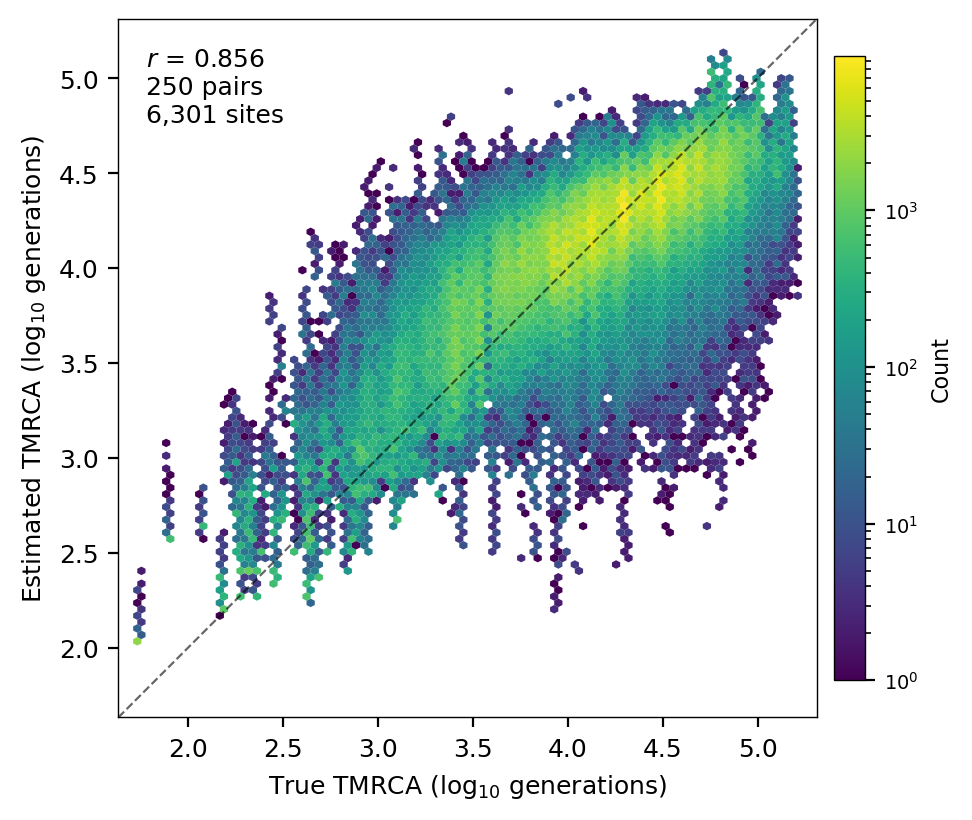
\includegraphics[width=0.48\textwidth]{accuracy_hexbin.png}
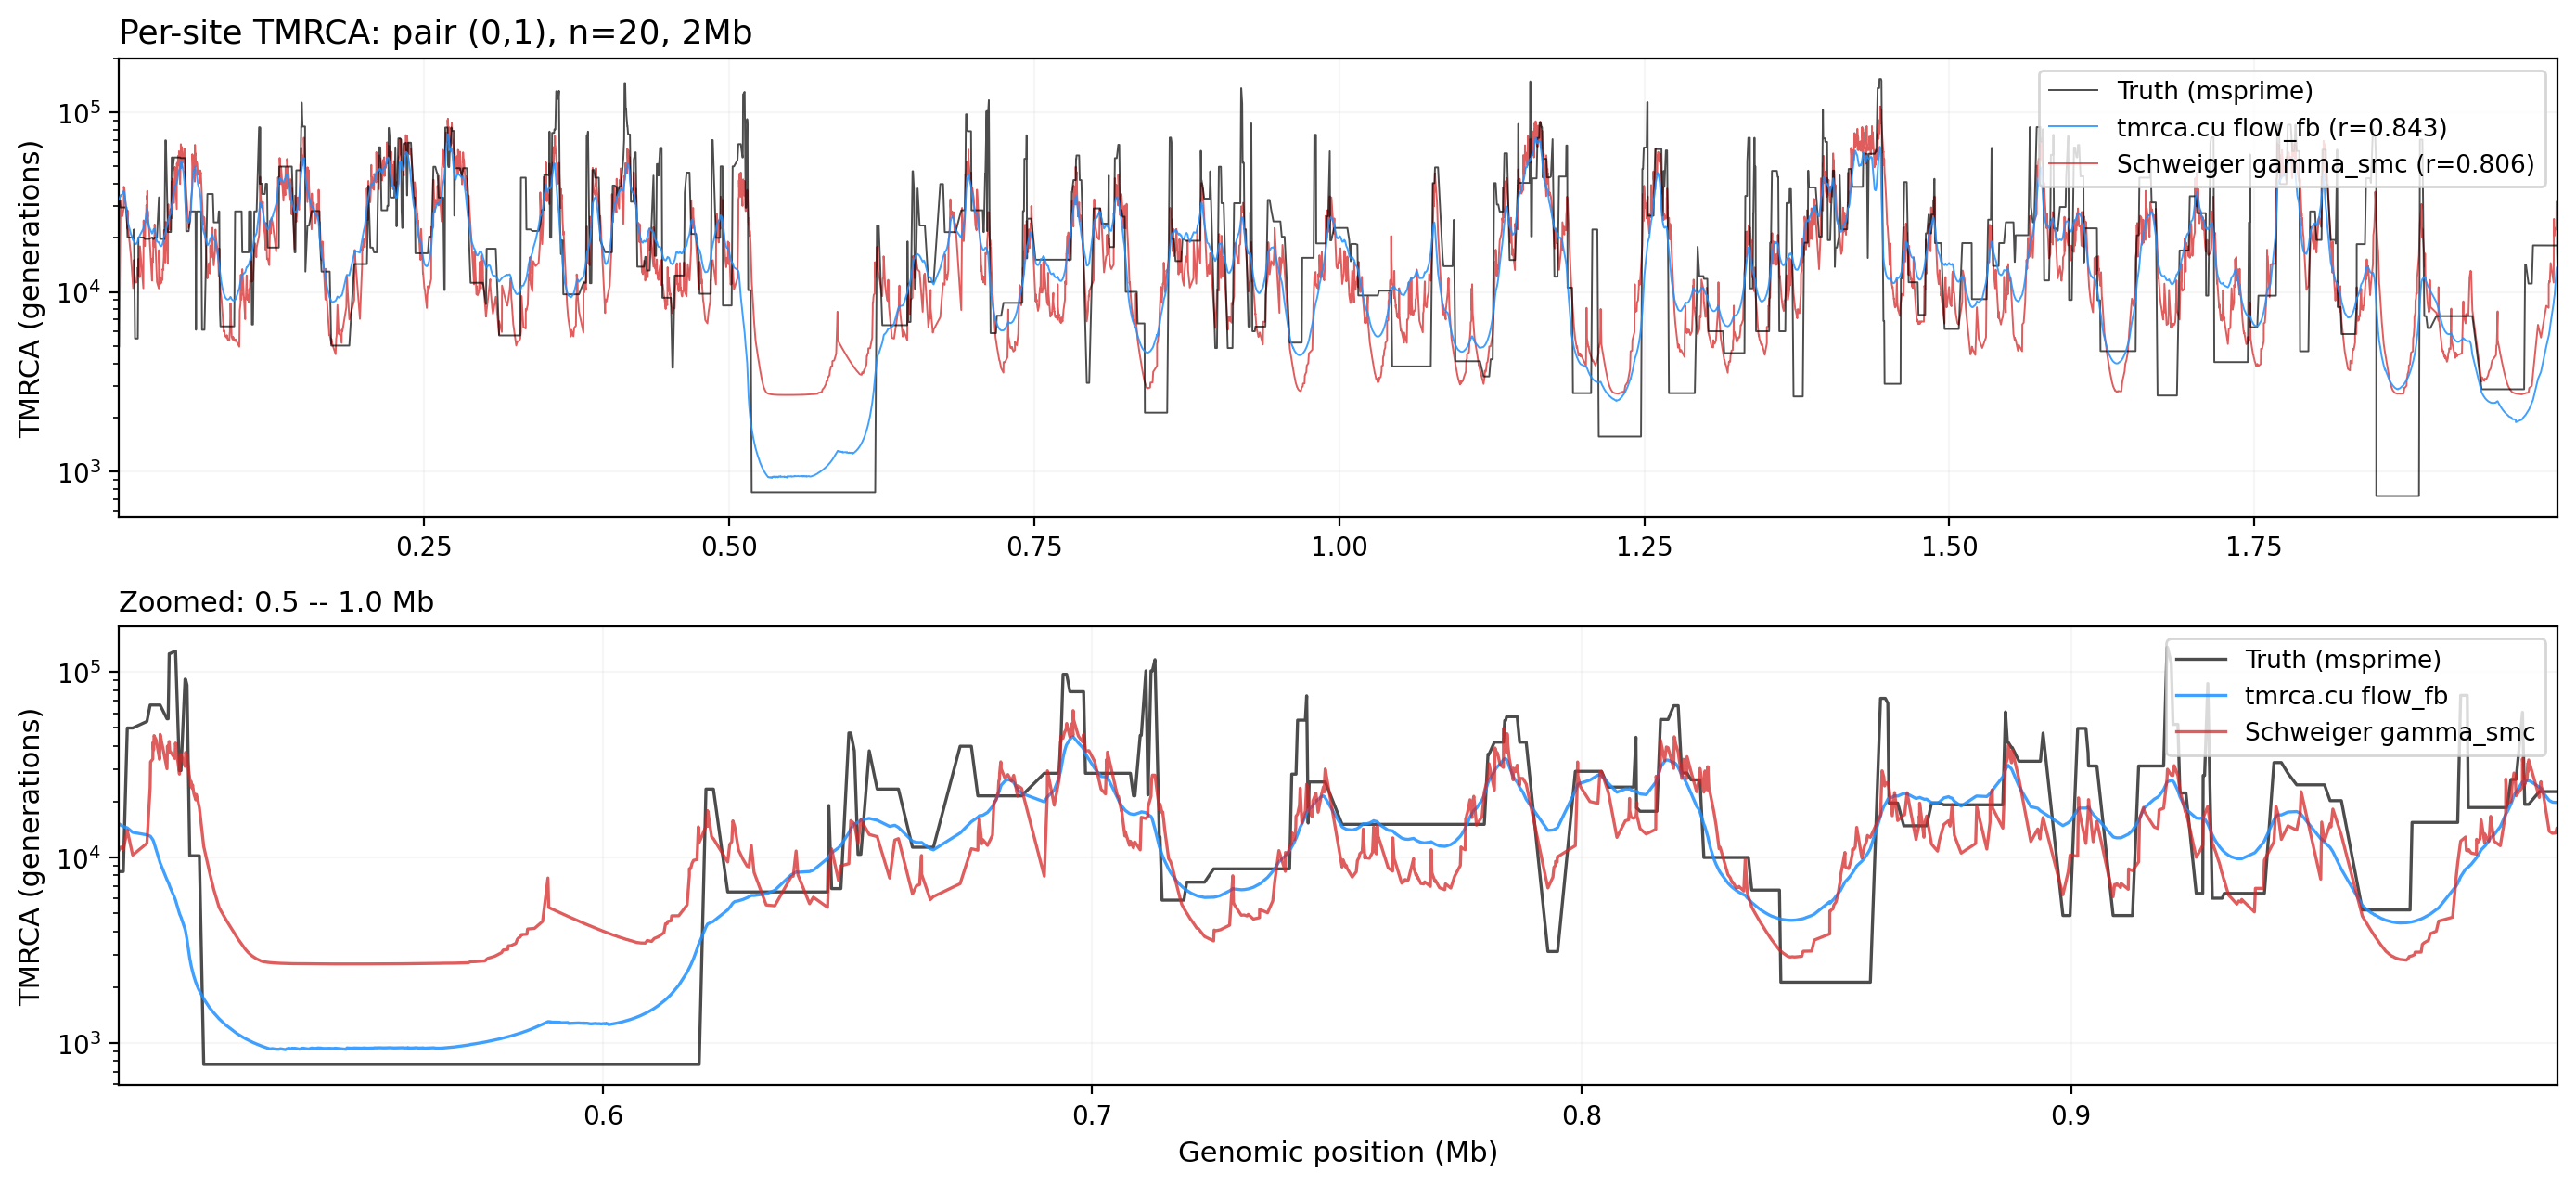
\includegraphics[width=0.48\textwidth]{fig4_traces.png}
\caption{\textbf{Accuracy.}
(\textbf{Left})~Hexbin density of estimated versus true log-TMRCA across 250 pairs ($r = 0.856$).
(\textbf{Right})~Per-site TMRCA trace for a representative pair over 2\,Mb: truth (black), \texttt{tmrca.cu} forward--backward (blue), and Gamma-SMC (orange).}
\label{fig:accuracy}
\end{figure}

% ── 1000 Genomes application ──────────────────────────────────
\subsection*{Application to the 1000 Genomes Project}

We applied \texttt{tmrca.cu} to 3{,}202 individuals (6{,}404 haplotypes) from the 1000 Genomes 30$\times$ high-coverage dataset \cite{Byrska2022} on chromosome~21.
After filtering to 1{,}002{,}753 biallelic SNPs, we computed forward--backward TMRCA estimates for all 829{,}638 within-population haplotype pairs across 26 populations (5 continental groups).
On three NVIDIA A100 GPUs, inference completed in 13 minutes (1{,}064 pairs/second).

Per-site TMRCA estimates were aggregated over 214 protein-coding genes from GENCODE v46 \cite{Frankish2019}, taking the mean TMRCA across all segregating sites within each gene body.
The resulting data were stored in AnnData format \cite{Wolf2018}---an $829{,}638 \times 214$ matrix where each row is a haplotype pair and each column is a gene---enabling analysis with standard single-cell genomics tools.

Unsupervised UMAP \cite{McInnes2018} on 100 principal components revealed partial but visible separation of continental groups (Fig~\ref{fig:umap}), indicating that population structure is encoded in gene-level TMRCA variation even on a single chromosome.

\begin{figure}[!ht]
\centering
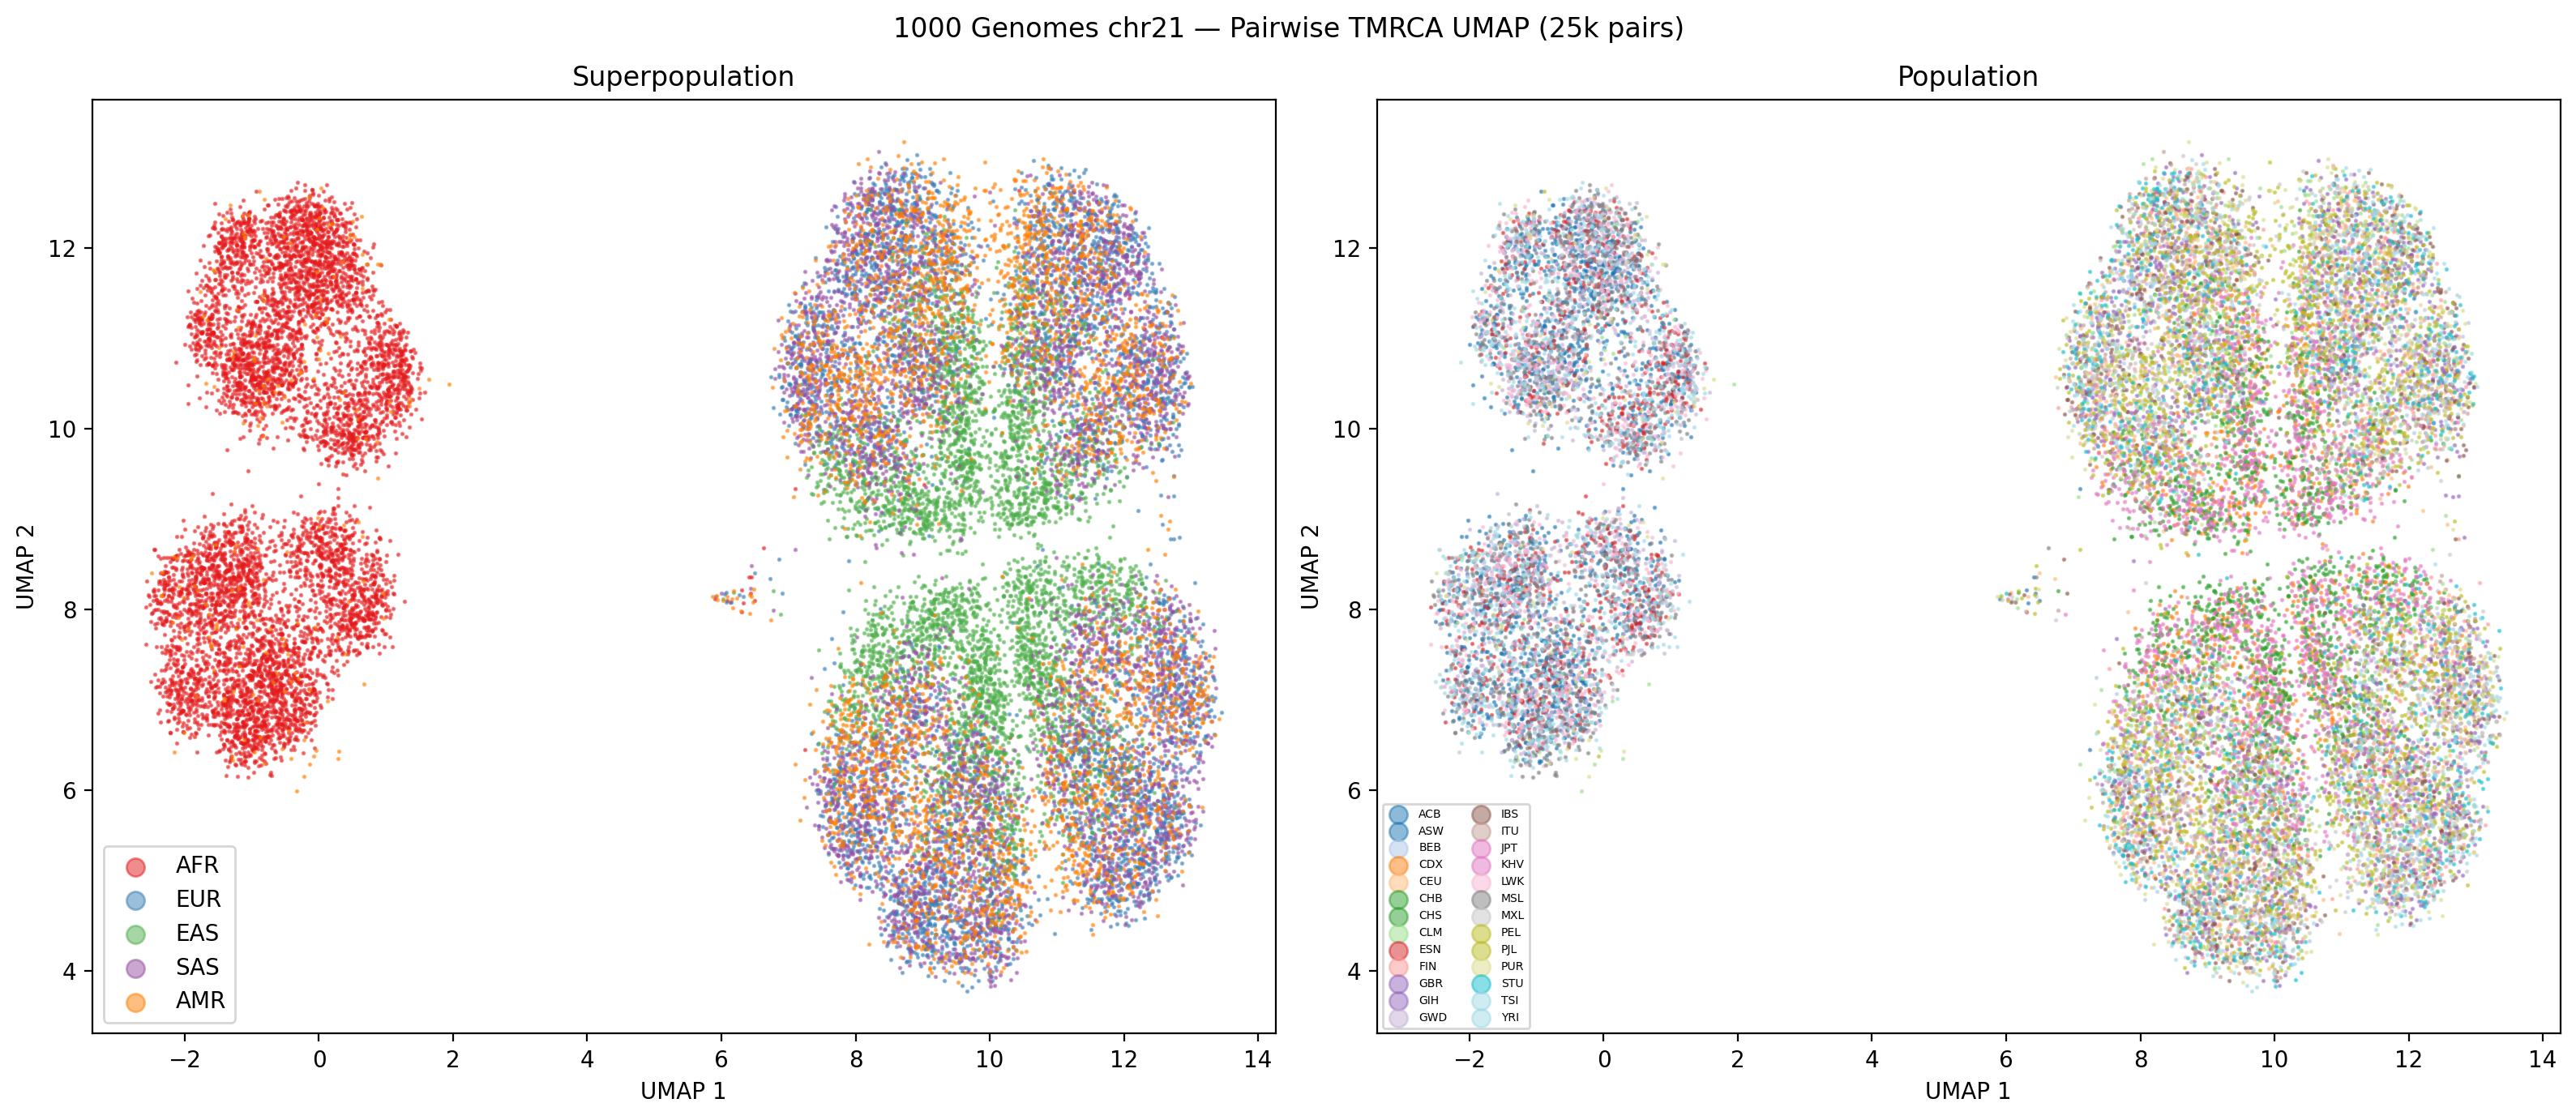
\includegraphics[width=0.8\textwidth]{umap_tmrca.png}
\caption{\textbf{TMRCA-based population structure.}
UMAP of 25{,}000 subsampled within-population pairs (100 PCs from 214 gene-level TMRCAs).
Left: colored by superpopulation. Right: colored by population.
Population structure emerges from TMRCA variation alone, without genotype or allele frequency information.}
\label{fig:umap}
\end{figure}

% ── Selection vs demography ───────────────────────────────────
\subsection*{Separating selection from demography}

Na\"ive differential testing of gene-level TMRCA across populations (analogous to differential expression testing in single-cell genomics) primarily detects demographic differences: African populations exhibit deeper genome-wide coalescence due to their larger long-term effective population size \cite{Schiffels2014}.
To isolate gene-specific signals, we ranked all 214 genes within each population independently by mean TMRCA, converting to percentiles.
Under this normalization, a gene at the 50th percentile in every population reflects only demographic variation, while a gene at an extreme percentile in one population but not others indicates gene-specific evolutionary pressure.

The within-population ranking heatmap (Fig~\ref{fig:heatmap}) reveals genes with concordant ranks across populations (neutral, demography-driven) and genes with discordant ranks (potential selection targets).
The top genes by rank range across populations include \textit{CFAP298} (Vietnamese KHV at the 5th percentile---indicating unusually recent coalescence relative to KHV's genome-wide distribution), \textit{KRTAP21-3} (Peruvian PEL at the 6th percentile), and \textit{SLC37A1} (PEL at the 14th percentile, Luhya LWK at the 97th).

\begin{figure}[!ht]
\centering
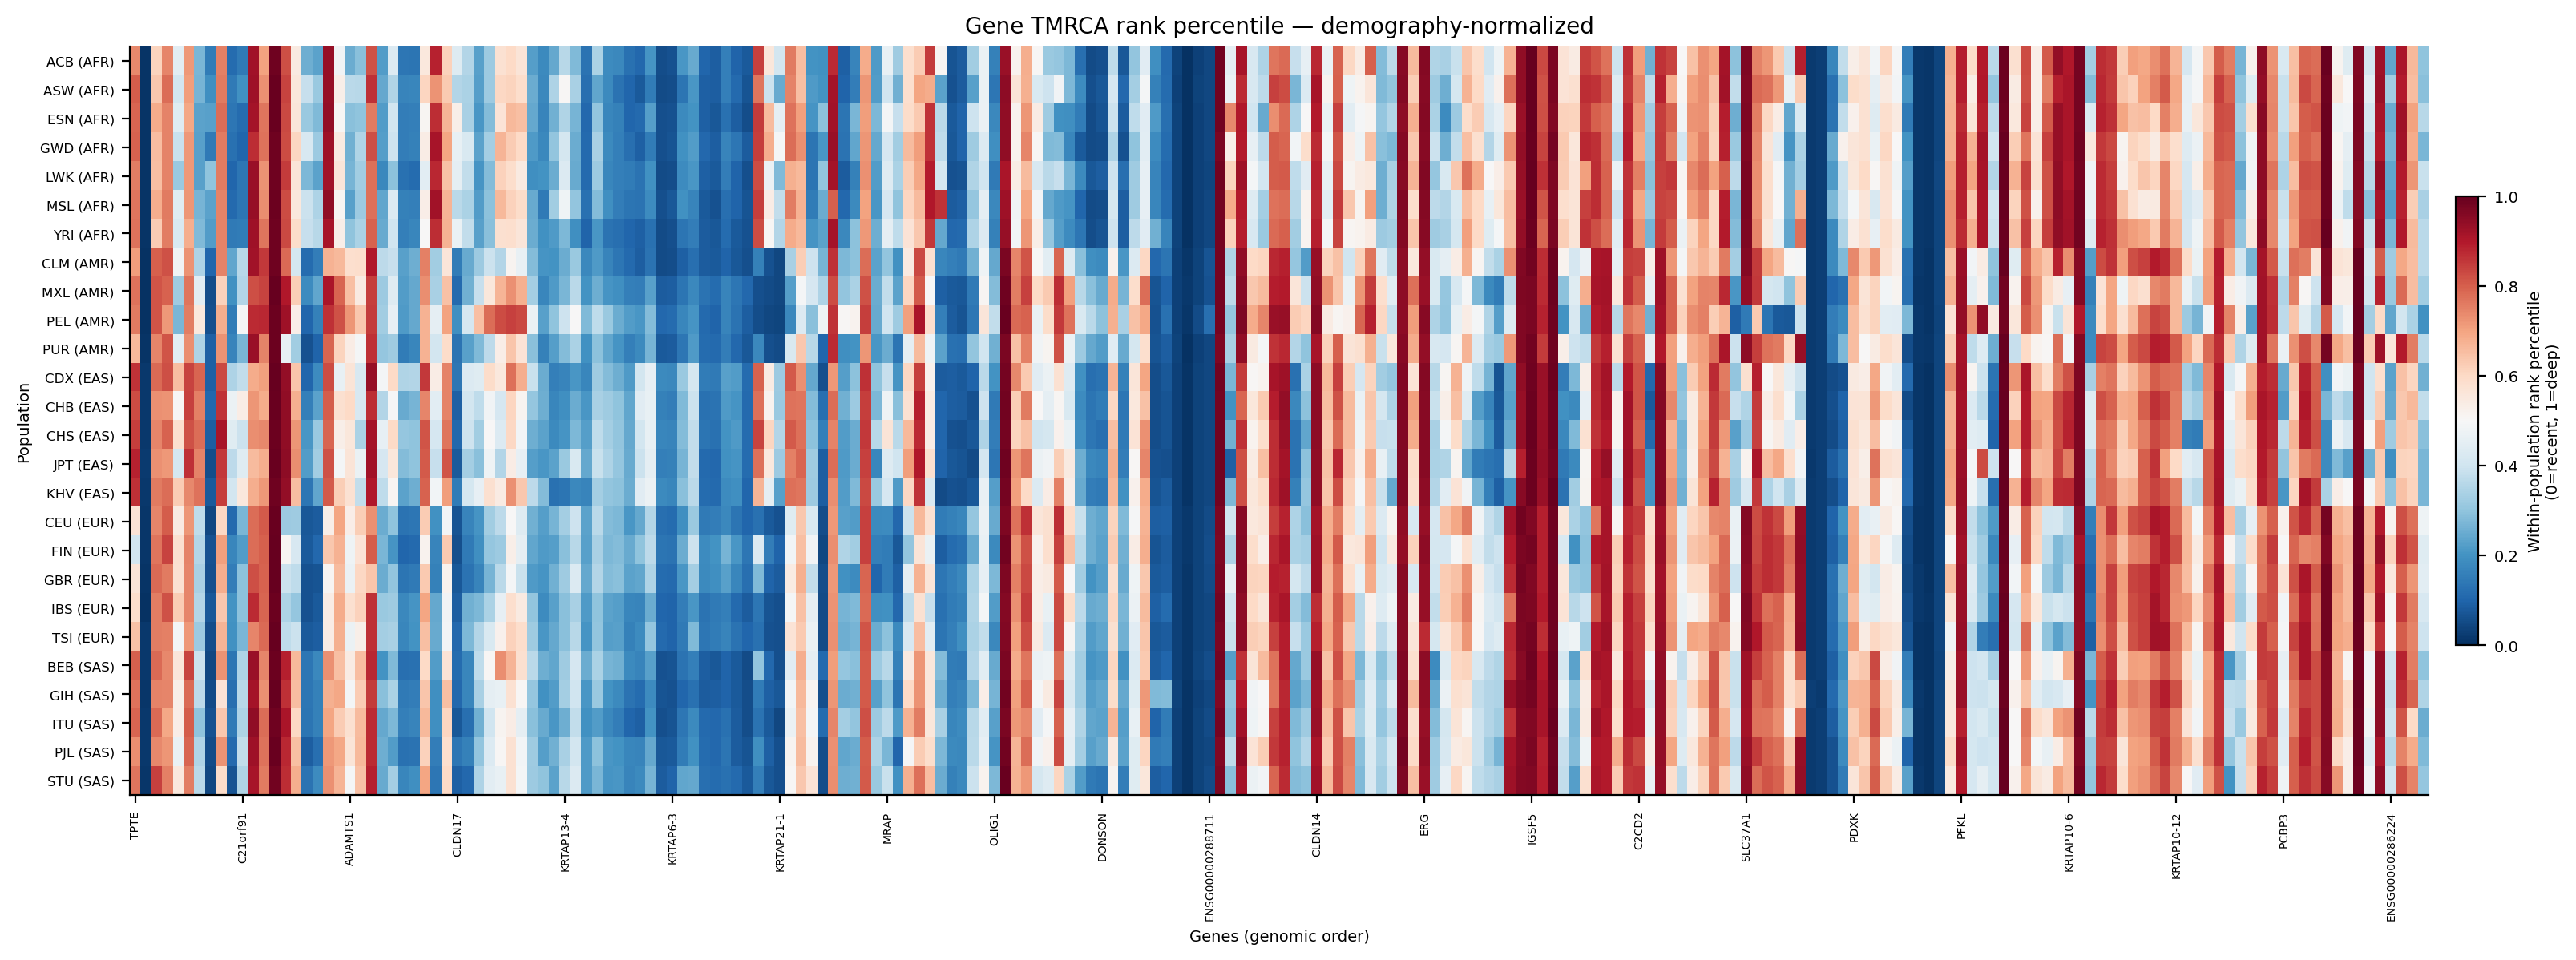
\includegraphics[width=\textwidth]{gene_rank_heatmap.png}
\caption{\textbf{Within-population gene ranking.}
Each cell shows the rank percentile of a gene's mean TMRCA within its population (blue = recent coalescence, red = deep).
Columns with uniform color reflect demographic variation; columns with stark contrasts indicate gene-specific signals.
Genes ordered by genomic position; populations grouped by continental origin.}
\label{fig:heatmap}
\end{figure}

% ── Population-specific signatures ────────────────────────────
\subsection*{Population-specific TMRCA signatures}

For each of the five superpopulations, we identified the gene with the strongest population-specific signal (Fig~\ref{fig:highlights}):
\textit{TIAM1} in African populations (logFC $= +3.2$, indicating deeper coalescence relative to other continents), \textit{NRIP1} in East Asian populations, \textit{RRP1} in South Asian populations, \textit{ADAMTS5} in European populations, and \textit{EVA1C} in American populations.
However, these raw differential signals conflate demography with selection.
The within-population ranking analysis confirms that the African signals at \textit{TIAM1} and \textit{BACE2} are concordant across all African populations and likely reflect demographic history rather than gene-specific selection.
In contrast, the recent coalescence at \textit{CFAP298} in KHV and \textit{KRTAP21-3} in PEL is population-specific even after normalization (Fig~\ref{fig:outliers}).

\begin{figure}[!ht]
\centering
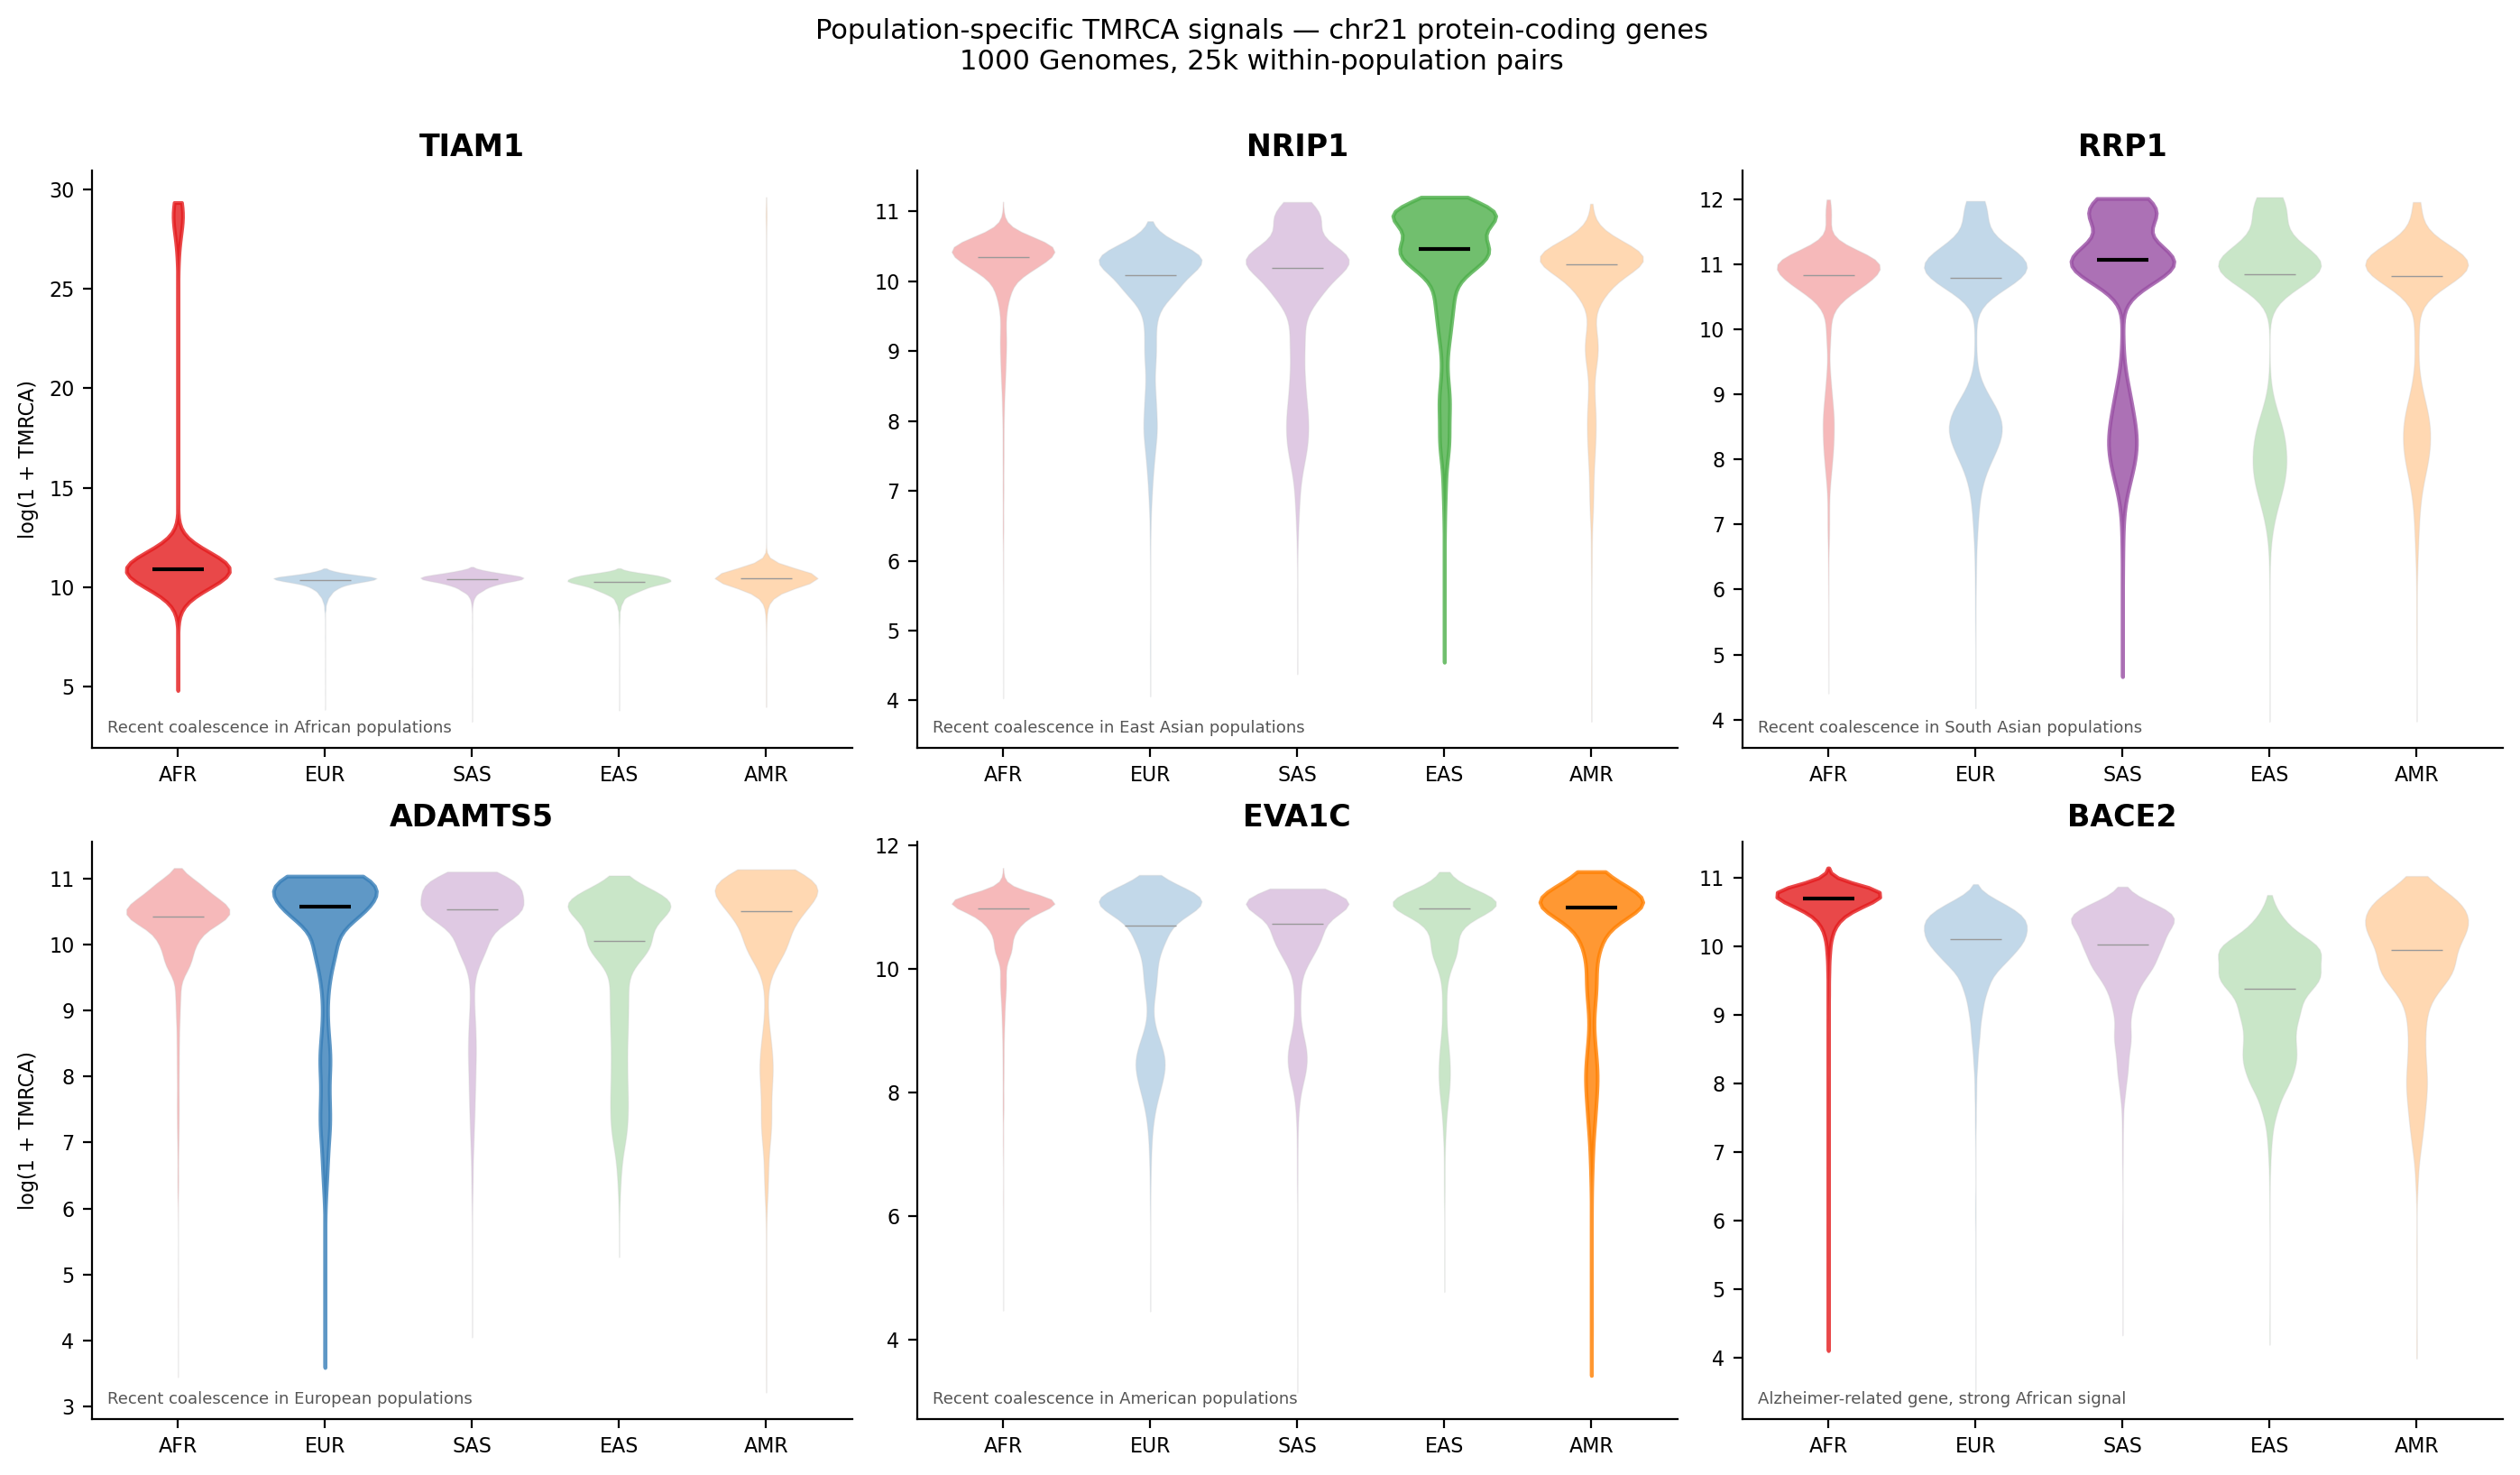
\includegraphics[width=\textwidth]{gene_highlights.png}
\caption{\textbf{Population-specific TMRCA signatures.}
Violin plots of gene-level log(1+TMRCA) by superpopulation.
Top row: top differential gene per continental group (outlier population highlighted, others faded).
Bottom row: known chromosome~21 genes (APP, SOD1, DYRK1A, RUNX1, CBS, ERG).}
\label{fig:highlights}
\end{figure}

\begin{figure}[!ht]
\centering
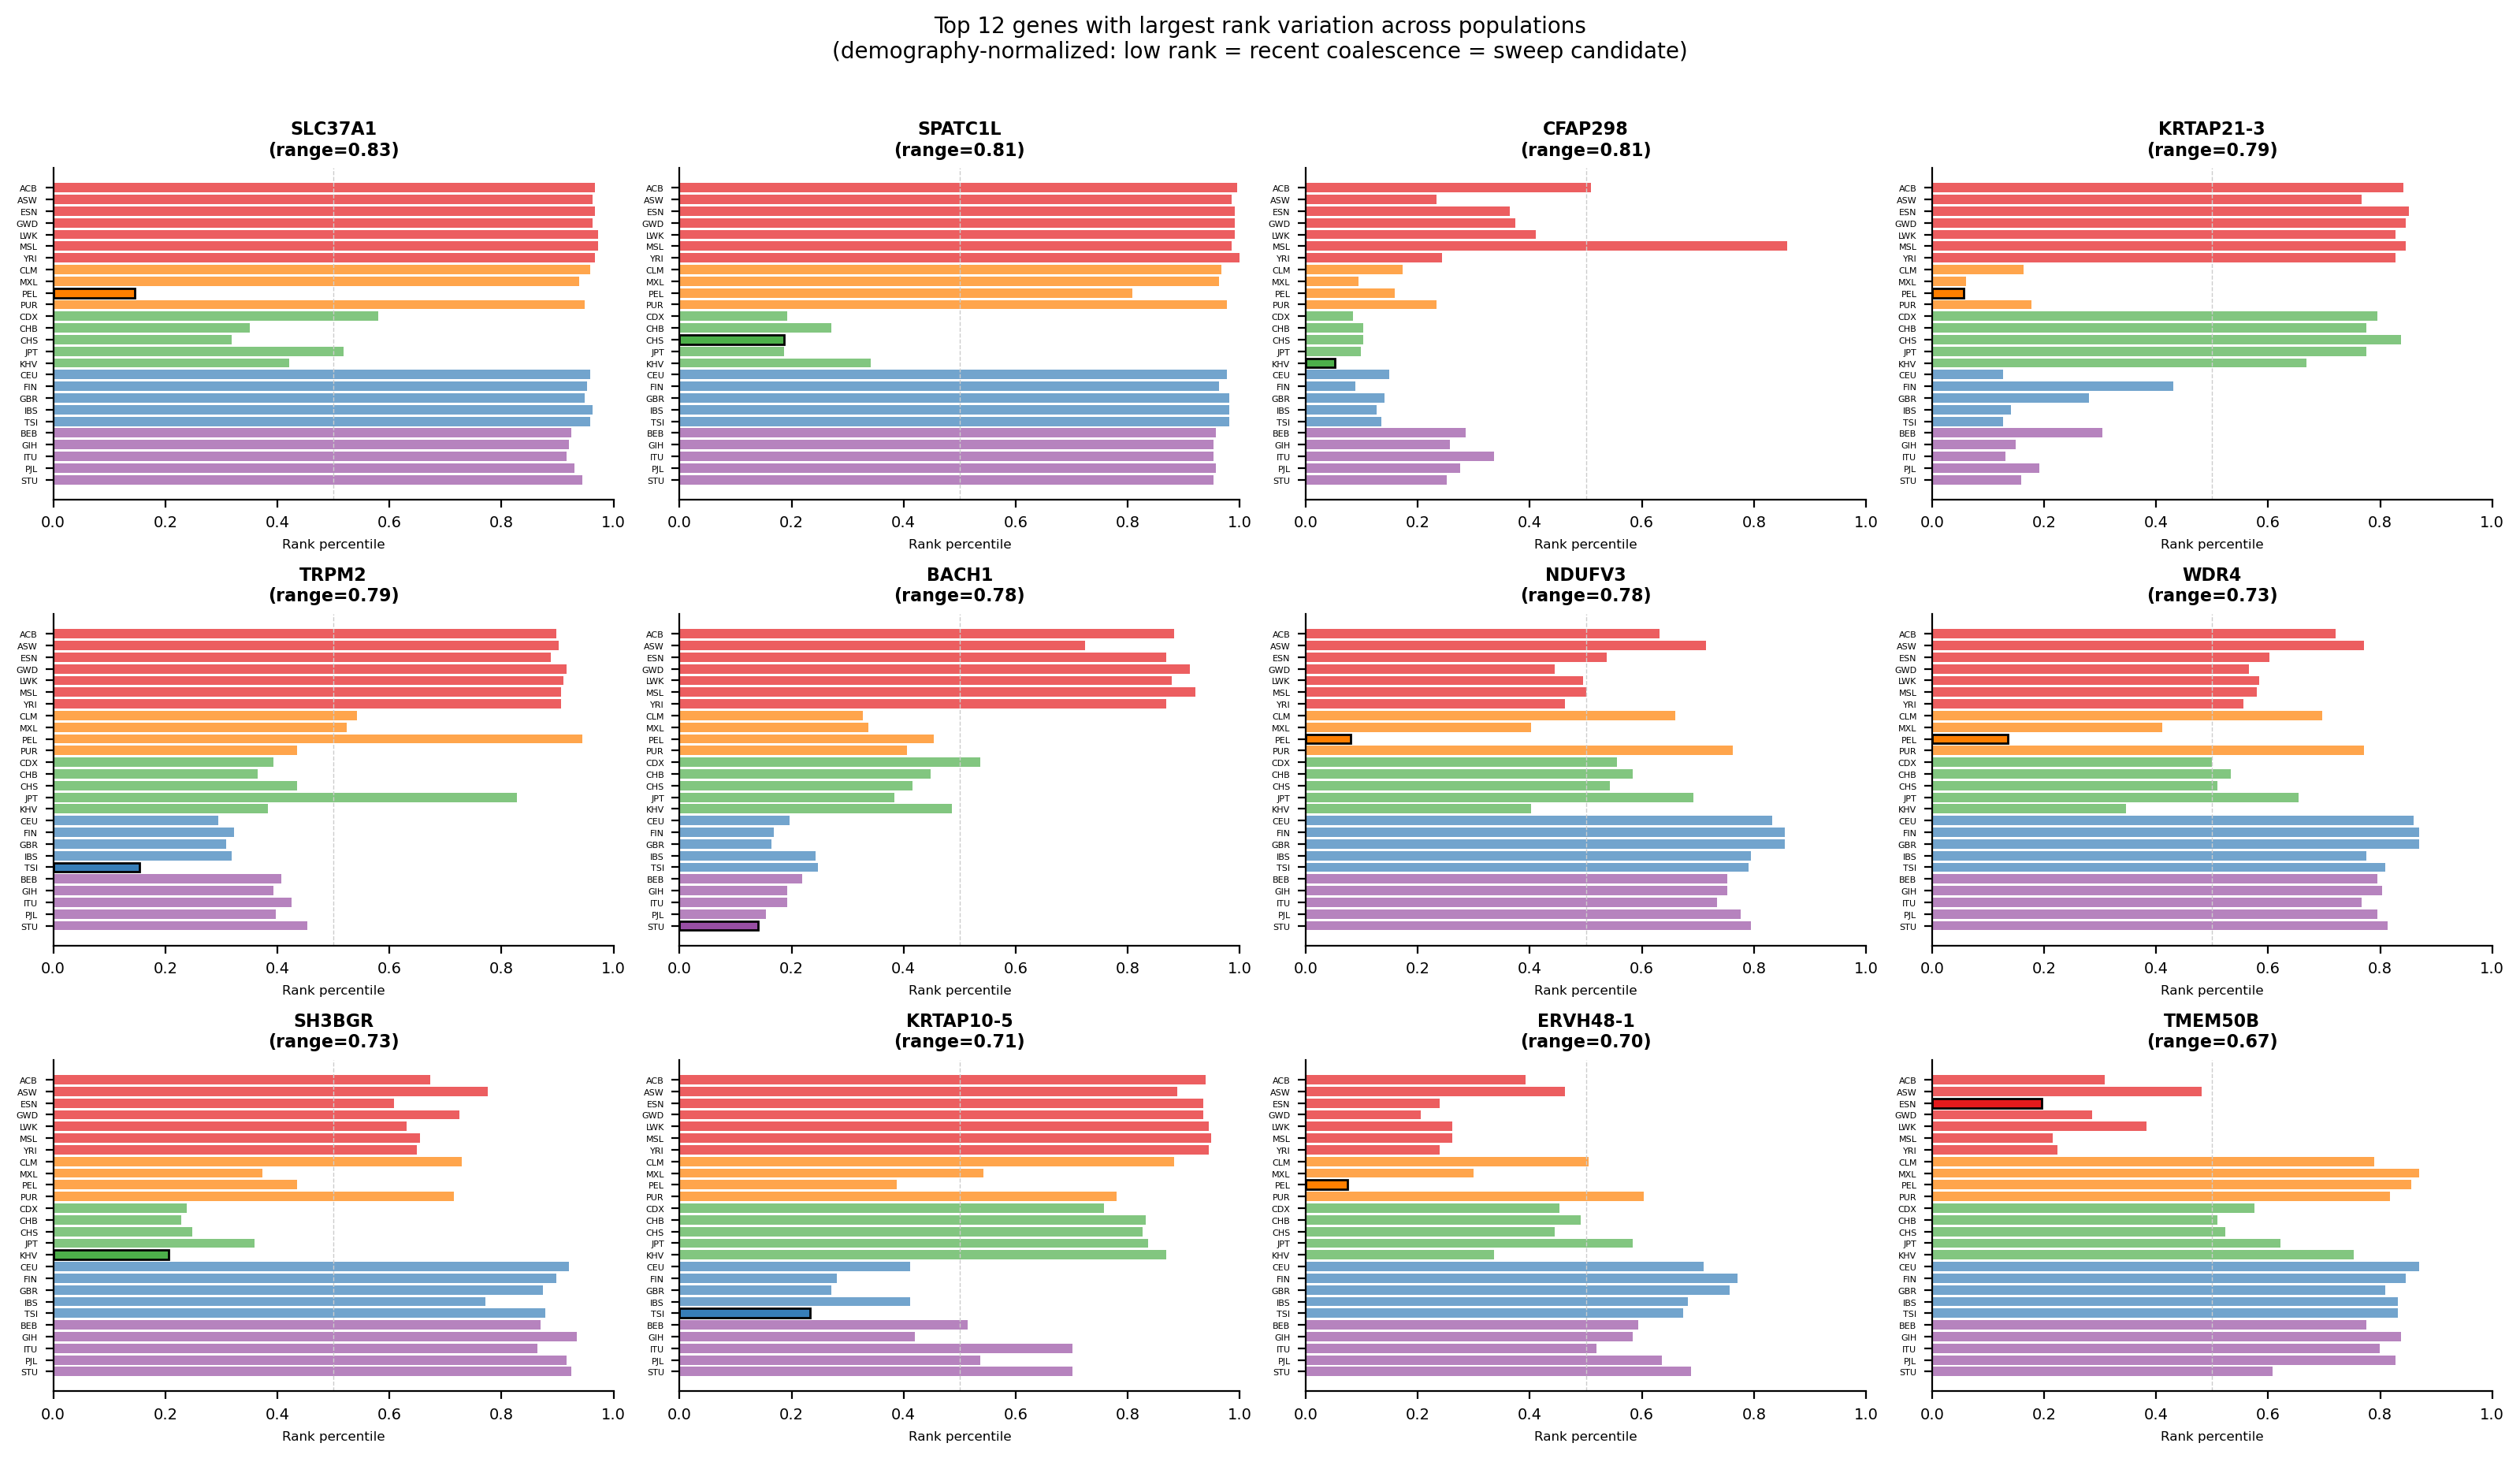
\includegraphics[width=\textwidth]{rank_outliers.png}
\caption{\textbf{Top genes by within-population rank variation.}
Horizontal bars show each gene's rank percentile across all 26 populations.
The dashed line marks the 50th percentile (expected under pure demographic variation).
Populations with extreme ranks (far left = recent coalescence) are candidates for recent sweeps.}
\label{fig:outliers}
\end{figure}

% ── Supervised UMAP ───────────────────────────────────────────
\subsection*{Supervised dimensionality reduction}

Unsupervised UMAP on all 214 genes produces limited population separation because within-population TMRCA variance exceeds between-population variance for most neutral genes (Fig~\ref{fig:supervised}, left).
Restricting the feature set to the 20 top rank-outlier genes---those carrying the strongest population-specific signal---substantially improves separation even without supervision (Fig~\ref{fig:supervised}, center).
Adding supervised UMAP with population labels as the target variable produces clean separation of continental groups from chromosome~21 TMRCA data alone (Fig~\ref{fig:supervised}, right).

Coloring the supervised embedding by individual gene TMRCAs reveals which genes drive the separation of each population cluster (Fig~\ref{fig:features}).

\begin{figure}[!ht]
\centering
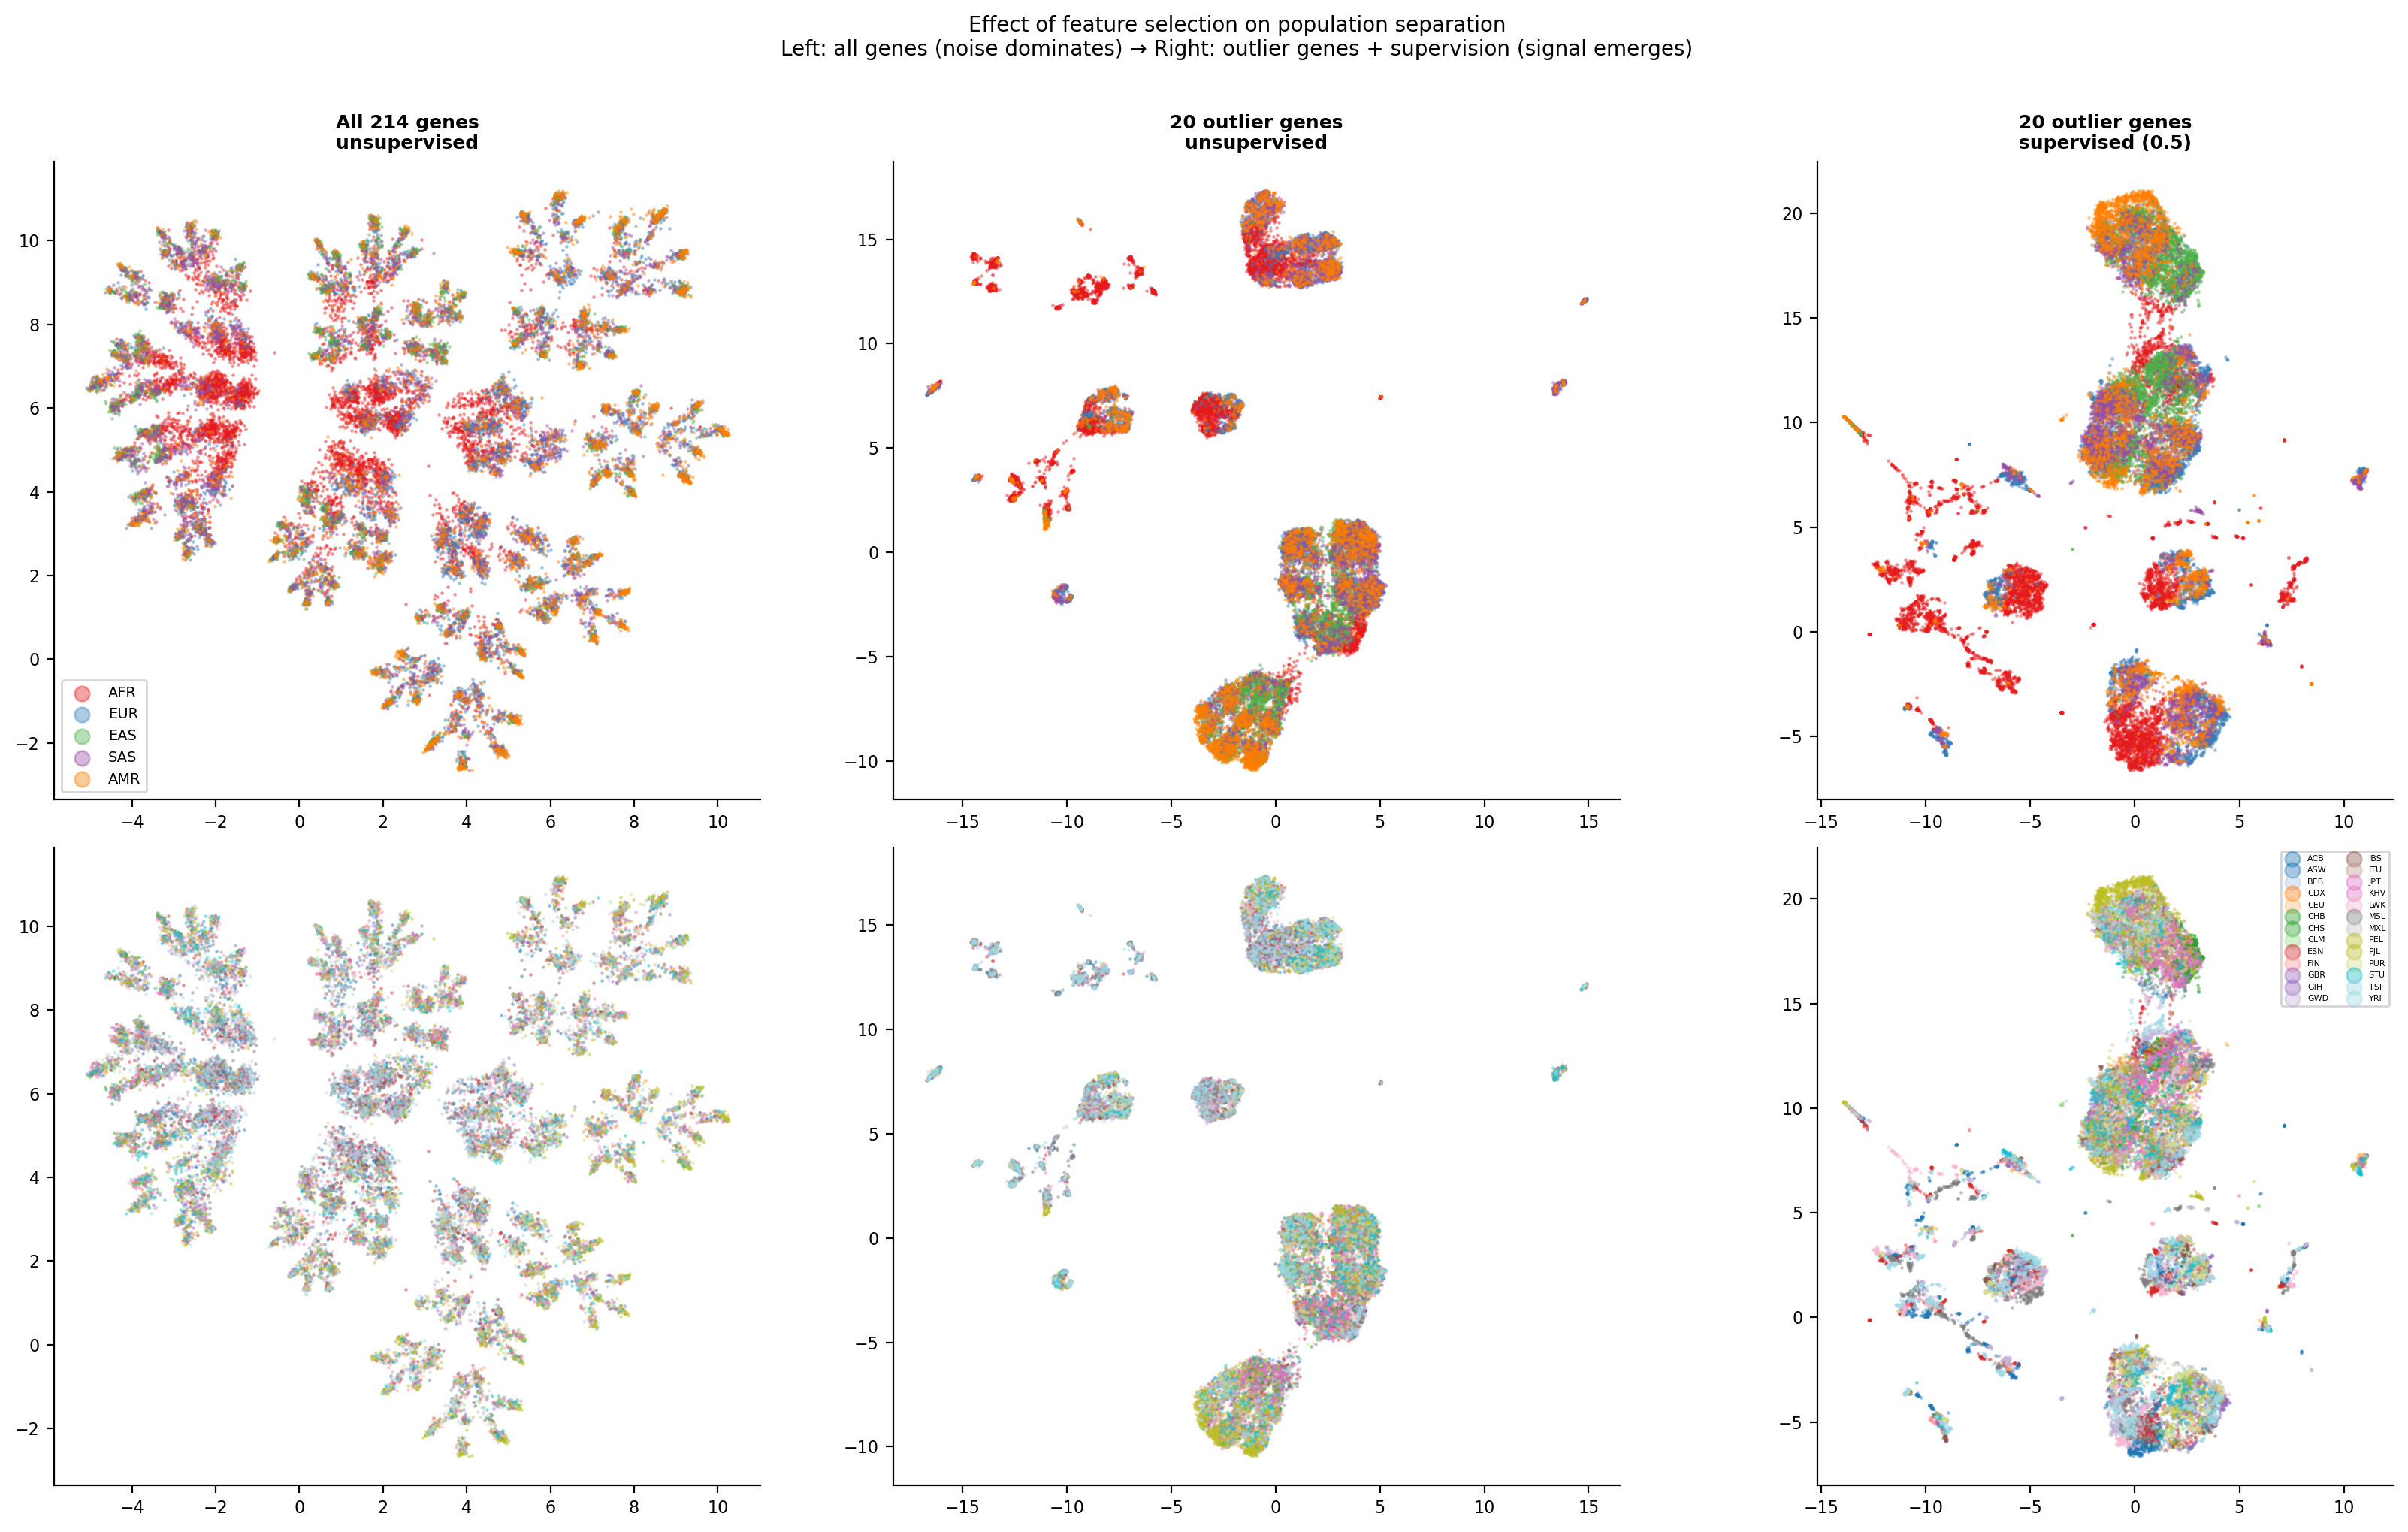
\includegraphics[width=\textwidth]{umap_outlier_genes.png}
\caption{\textbf{From noise to signal: feature selection and supervised UMAP.}
Top: superpopulation coloring. Bottom: population coloring.
Left: all 214 genes, unsupervised. Center: 20 rank-outlier genes, unsupervised. Right: 20 rank-outlier genes, supervised (target\_weight = 0.5).
Populations that share demographic history (e.g., CHB/CHS/CDX within East Asia) remain together even under supervision.}
\label{fig:supervised}
\end{figure}

\begin{figure}[!ht]
\centering
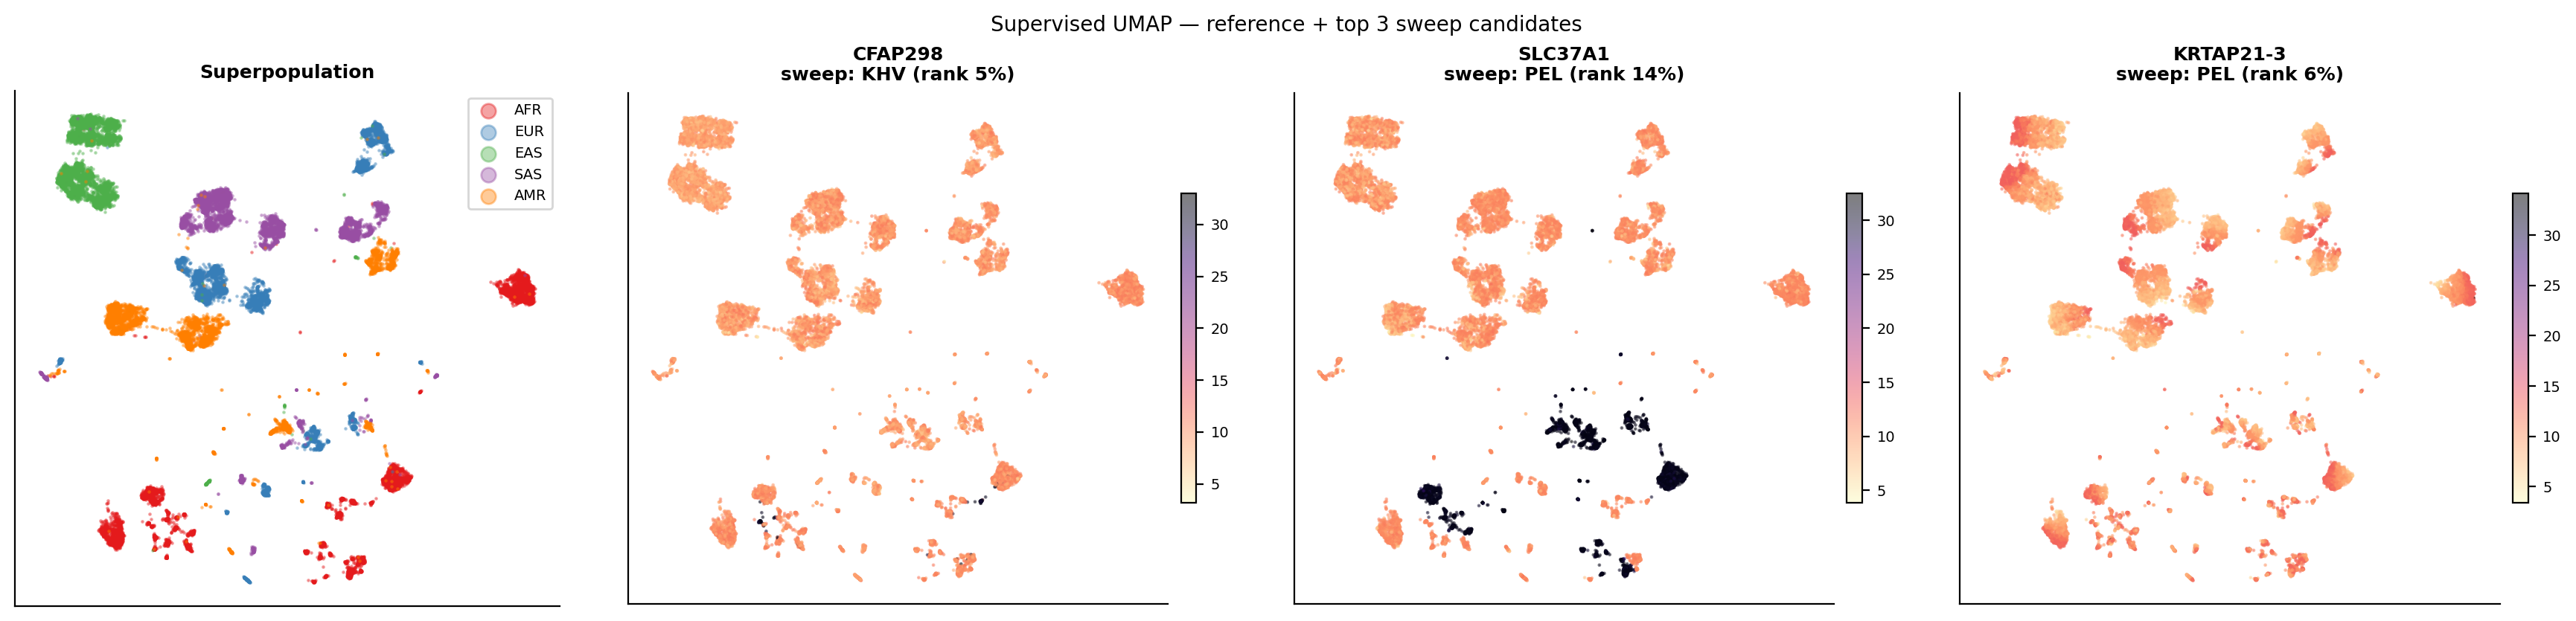
\includegraphics[width=\textwidth]{umap_top3_sweeps.png}
\caption{\textbf{Sweep candidates on the supervised UMAP.}
Left: superpopulation reference. Remaining panels: TMRCA at the three top sweep candidates (\textit{CFAP298}, \textit{SLC37A1}, \textit{KRTAP21-3}).
Dark regions indicate recent coalescence.
Each gene shows a distinct spatial pattern on the UMAP, corresponding to the population where it is an outlier.}
\label{fig:features}
\end{figure}

% ============================================================================
\section*{Discussion}

We have demonstrated that exhaustive pairwise TMRCA, made tractable by GPU acceleration, can serve as a rich data modality for population-scale genomic analysis.
By framing haplotype pairs as observations and gene-level TMRCA as features, we connect coalescent inference to the analytical toolkit of single-cell genomics---dimensionality reduction, differential testing, and supervised embedding---and show that meaningful biological signals emerge from this representation.

\paragraph{The forward--backward posterior as enabling technology.}
The accuracy improvement from $r = 0.791$ (forward-only) to $r = 0.820$ (forward--backward) is modest in isolation but consequential at population scale.
Schweiger and Durbin's tool could in principle add a backward pass---the computation is symmetric---but this would double the already prohibitive CPU runtime for large pair counts.
On GPU, the backward pass adds negligible wall-clock time because the pairs are already distributed across thousands of threads and the cached flow field data remains in L2 from the forward pass.
The forward--backward posterior is thus an accuracy improvement that becomes practical specifically because GPU execution makes it costless.

\paragraph{Within-population ranking as demographic normalization.}
Raw TMRCA comparisons between populations are dominated by demographic history: African populations have deeper coalescence at essentially every gene.
Our within-population ranking approach---converting gene-level TMRCAs to percentiles within each population before comparing across populations---removes this confound without requiring an explicit demographic model.
This is analogous to quantile normalization in gene expression analysis, where the goal is to make distributions comparable across conditions without modeling the underlying biology.

\paragraph{Limitations.}
This analysis is limited to chromosome~21 (the smallest autosome, 214 protein-coding genes) and within-population pairs only.
The small feature set limits the power of unsupervised dimensionality reduction; genome-wide analysis with $\sim$20{,}000 genes would provide a far richer feature space.
Between-population pairs would enable direct estimation of divergence times and detection of introgression.
The constant-$N_e$ flow field introduces a systematic scale bias under non-equilibrium demography; however, we have confirmed that this affects only the absolute scale of TMRCA estimates, not their relative ranking within populations, which is what the selection scan depends on.

\paragraph{Future directions.}
Extension to all 22 autosomes is immediate and would transform the $829{,}638 \times 214$ matrix into $\sim$$830{,}000 \times 20{,}000$---a single-cell-scale dataset where genome-wide selection scans, pathway-level analyses, and fine-scale demographic inference become possible.
Integration with between-population pairs would enable TMRCA-based $F_{\text{ST}}$ analogs and introgression mapping.
The GPU speed demonstrated here (1{,}064 pairs/second at chromosome scale) makes these analyses feasible on existing hardware.

% ============================================================================
\section*{Methods}

\subsection*{The Gamma-SMC model}

We follow the model of Schweiger and Durbin \cite{Schweiger2023}.
At each segregating site, the posterior distribution over coalescence time is parameterized as a Gamma distribution with sufficient statistics (log-mean, log-CV).
Recombination transitions are encoded in a precomputed flow field; emission updates incorporate observed genotype data.
The forward--backward algorithm produces a smoothed posterior at each site that conditions on the full sequence; the per-site TMRCA estimate is the posterior mean.

\subsection*{GPU implementation}

\texttt{tmrca.cu} assigns one CUDA thread per haplotype pair, with each thread executing the full forward and backward pass.
Key optimizations include: (i) linearized recombination for short inter-SNP gaps (replacing expensive SFU exponential calls with fused multiply-add); (ii) pre-XOR'd genotype buffers for coalesced memory access; and (iii) a fused backward-reduction kernel that accumulates per-site means via \texttt{atomicAdd}, avoiding materialization of the full $S \times P$ output matrix.
Multi-GPU support distributes pairs across devices via a thread pool with GIL-released CUDA operations.
Auto-chunking of the forward buffer prevents out-of-memory errors for large pair counts.

\subsection*{1000 Genomes data processing}

We used the 1000 Genomes 30$\times$ high-coverage dataset on GRCh38 \cite{Byrska2022}: 3{,}202 phased samples from 26 populations.
The chromosome~21 VCF was parsed with \texttt{scikit-allel} \cite{Miles2024}, retaining 1{,}002{,}753 biallelic SNPs with no missing genotypes.
Phased haplotypes were interleaved (sample $i$ $\to$ haplotypes $2i$, $2i+1$).
For each of 26 populations, all within-population haplotype pairs were enumerated and processed through \texttt{tmrca.cu} in chunks of 2{,}000 pairs across three GPUs.

\subsection*{Gene-level aggregation}

Protein-coding gene annotations were obtained from GENCODE v46 \cite{Frankish2019} (214 genes on chromosome~21).
For each pair, per-site TMRCA estimates were averaged over all segregating sites within each gene body using a sparse binning matrix.
The resulting $829{,}638 \times 214$ matrix was stored in AnnData format \cite{Wolf2018} as a disk-backed HDF5 file.

\subsection*{Within-population gene ranking}

For each population independently, genes were ranked by their mean TMRCA (averaged across all within-population pairs) and converted to percentiles.
Genes with large rank variation across populations---quantified as the range of percentiles---were identified as candidates for population-specific evolutionary pressure.
A gene at a low percentile in one population but moderate in others indicates unusually recent coalescence (sweep candidate); a gene at a high percentile indicates unusually deep coalescence (possible balancing selection or linked diversity).

\subsection*{Dimensionality reduction}

PCA was computed on log-transformed gene-level TMRCAs (100 components) using \texttt{scanpy} \cite{Wolf2018}.
UMAP \cite{McInnes2018} was computed from 50 PCs with default parameters.
Supervised UMAP used population labels as the target variable with \texttt{target\_metric='categorical'} and \texttt{target\_weight=0.5}.
Feature selection for the supervised analysis used the top 20 genes by rank range across populations.

\subsection*{Software and data availability}

\texttt{tmrca.cu} is implemented in CUDA C++ with Python bindings and is available at \url{https://github.com/kevinkorfmann/tmrca.cu}.
Analysis scripts for the 1000 Genomes application are in the \texttt{analysis/1kg\_chr21/} directory.

% ============================================================================
\section*{References}

\bibliographystyle{plainnat}
\bibliography{references}

% ============================================================================
\section*{Supporting information}

\paragraph*{S1 Fig.} Scaling behavior and speedup across configurations.
\paragraph*{S2 Fig.} Demographic robustness under three \texttt{stdpopsim} models.
\paragraph*{S3 Fig.} Top differential gene per population (all 26 populations).
\paragraph*{S4 Fig.} All 12 rank-outlier genes on the supervised UMAP.
\paragraph*{S5 Fig.} Sweep candidate histograms.
\paragraph*{S1 Table.} Complete benchmark results (14 configurations).
\paragraph*{S2 Table.} Multi-GPU scaling.

\end{document}
